\section{BJT in Saturation Mode}
Change the value of \textbf{R1 to 1k} and run the simulation again. Capture the simulation results and explain the values of $I_B, I_C, V_{CE}$. The default transistor gain is $\beta = 100$, and the saturated voltage $V_{CE(Sat)} = 0.65V$ and $V_{BE} = 0.7V$.

\textbf{\textit{Your image goes here:}}\\
% 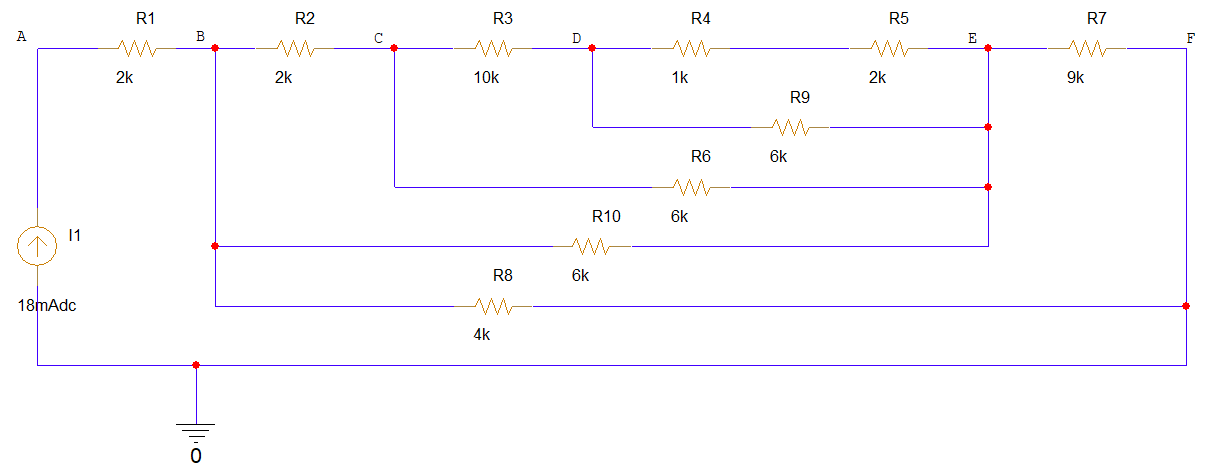
\includegraphics[]{graphics/ex1/f1.PNG}
\vspace{6cm}

Kết quả trong PSpice được giải thích như sau:

\begin{itemize}
    \item Áp dụng định luật Ohm, $I_B = \frac{V_{BB} - V_{BE}}{R_1} = \frac{5 - 0.7}{1000} =  4.3$ mA
    \item Giả sử transistor ở vùng tích cực, $I_C = \beta \cdot I_B = 100  \cdot 4.3 = 0. 43$ A  
    \item Cuối cùng, để kiểm chứng giả định trên, $V_{CE} = V_{CC} - I_C \cdot R_2 = 10 - 0.43 \cdot 100 = -32$ V 
\end{itemize}

Vì $V_{CE} < 0$, giả định trên là sai. Con transistor ở vùng bão hòa. Do đó, $I_C$ được xác định như sau:\\

$$I_C = \frac{V_{CC} - V_{CE(Sat)}}{R_2} = \frac{10 - 0.65}{100} = 93.5 mA$$

